\section{Wakefields, Impedances and Beam Dynamics Effects}

\section{Theoretical Background of Wakefields and Impedances}

%
% Explaination of the concept of wakefields (the source and witness particle), oscillating electric fields
% induced by a charged particle. Longitudinal and Transverse wakefields
% Relation of wakefields to impedance by fourier transform - also distinction between wakefields (bunch phenomena), wakefunction (single particle/structure property)
% loss factor/kick factor
%
% The derivation of Panowsky-Wenzel and the relation between longitudinal and transverse impedance
% Break up of transverse impedance into dipolar and quadrupolar and relative positions of particles
% 
% Simple Examples
% Resistive Wall
%
% Geometric impedance 
% of a pillbox cavity
%
%
%
%
%
%
%
%
%

\subsection{Resistive Wall Impedance}

\subsection{Geometric Impedance}

\section{Examples of Effects}

\subsection{Beam Induced Heating}

One consequence of the presence of longitudinal impedance is the phenomena of beam-induced heating. First we should consider the so called parasitic loss of a charged particle interacting with a generic impedance[ref Chao/Ng];

\begin{equation}
\Delta E = -2\pi e^{2}N_{b}\int^{\infty}_{-\infty} d\omega \left| \lambda \left( \omega \right)  \right|^{2} Z_{\parallel} \left( \omega \right)
\end{equation}

where $\Delta E$ is the energy loss per pass per particle, $e$ is the charge per particle, $N_{b}$, $\omega$ the frequency, $\lambda$ the line density of the bunch and $Z_{\parallel}$ the longitudinal impedance of the object being traversed.
																
Due to the decay of the wakefields induced by this energy loss, this energy must eventually be lost to the device causing the impedance (valid below the cutoff frequency of the machine beam pipe). Therefore we can assume that the energy loss from the particles is absorbed by the surrounding structure. Summing over all particles in a bunch we can therefore obtain a sum of the energy loss;

\begin{equation}
\Delta E_{bunch} = 2\pi \left( eN_{b}   \right)^{2} \int^{\infty}_{-\infty} d\omega \left| \lambda \left( \omega \right)  \right|^{2} Z_{\parallel} \left( \omega \right)
\end{equation}

As often we must deal with machines storing multiple bunches, for these we simply multiply the energy loss per bunch by the number of stored bunches;

\begin{equation}
\Delta E_{buunches} = 2\pi \left( eN_{b}   \right)^{2}n_{bunch} \int^{\infty}_{-\infty} d\omega \left| \lambda \left( \omega \right)  \right|^{2} Z_{\parallel} \left( \omega \right)
\end{equation}

where $n_{bunch}$ is the number of bunches in the machine. If we assume a revolution frequency $f_{rev}$ we thus get a power loss of;

\begin{align}
P_{loss}  = & \Delta E_{bunches} f_{rev}\nonumber \\  
 = & 2\pi f_{rev} \left( eN_{b}   \right)^{2}n_{bunch} \int^{\infty}_{-\infty} d\omega \left| \lambda \left( \omega \right)  \right|^{2} Z_{\parallel} \left( \omega \right) \nonumber  \\ 
 = & \omega_{rev} \left( eN_{b}   \right)^{2}n_{bunch} \int^{\infty}_{-\infty} d\omega \left| \lambda \left( \omega \right)  \right|^{2} Z_{\parallel} \left( \omega \right) \nonumber \\
 = & \omega_{rev} \left( eN_{b}   \right)^{2}n_{bunch} \int^{\infty}_{-\infty} d\omega \left| \lambda \left( \omega \right)  \right|^{2} \left( \Re{}e \left( Z_{\parallel} \left( \omega\right) + \Im{}m Z_{\parallel} \left( \omega\right) \right) \right).
\end{align}
 
As $\Re{}e\left(Z_{\parallel} \left( \omega\right)\right)$ is an even function and $\Im{}m\left(Z_{\parallel} \left( \omega\right)\right)$ is an odd function, we see that

\begin{equation}
P_{loss}   =  \omega_{rev} \left( eN_{b}   \right)^{2}n_{bunch} \int^{\infty}_{0} 2 d\omega \left| \lambda \left( \omega \right)  \right| ^{2}  \Re{}e \left( Z_{\parallel} \left( \omega\right)  \right).
\end{equation}

Next we make a change of the variable of integration $\omega = n{bunch}\omega_{rev}$;

\begin{equation}
P_{loss}   =  \omega_{rev} \left( eN_{b}   \right)^{2}n_{bunch}^{2} \int^{\infty}_{0} 2 d\omega_{rev} \left| \lambda \left( \omega_{rev}n_{bunch} \right)  \right|^{2}  \Re{}e \left( Z_{\parallel} \left( \omega_{rev}n_{bunch}\right)  \right).
\end{equation}

We can subsequently change to a sum formalism to obtain

\begin{align}
P_{loss} & = \left( \omega_{rev}eN_{b}n_{bunch}  \right)^{2} \displaystyle\sum\limits_{n = 0}^{\infty} \left( 2 \left| \lambda \left( \omega_{rev}n_{bunch} \right)  \right|^{2}  \Re{}e \left( Z_{\parallel} \left( \omega_{rev}n_{bunch}\right) \right) \right) \label{ean:heating-gen} \\
P_{loss} & = \left( \omega_{rev}eN_{b}n_{bunch}  \right)^{2} \displaystyle\sum\limits_{n = 0}^{\infty} \left( 2 \left| \lambda \left( \omega_{0} \right)  \right|^{2}  \Re{}e \left( Z_{\parallel} \left( \omega_{0}\right) \right) \right)
\end{align}

where $\omega_{0} = 2\pi f_{0}$, $f_{0} = \frac{1}{\tau_{b}}$ and $\tau_{b}$ is the bunch spacing.

Often we define the impedance of a structure using a resonator model, where the impedance is defined as

\begin{equation}
Z_{\parallel}\left( \omega \right) = \frac{R_{s}}{1 + Q\left( \frac{\omega_{res}}{\omega} - \frac{\omega}{\omega_{res}} \right)}
\end{equation}

where $R_{s}$ is the shunt impedance, $Q$ the quality factor, $\omega$ the frequency and $\omega_{res}$ the resonant frequency

It is often useful to make the distinction between heating due to a broadband impedance (interacts with many spectral lines) and a narrowband impedance (interacts with only one spectral line). This is due to the different ways in which the heating due to these impedances changes with increasing or decreasing the number of bunches in a machine.

\subsubsection{Heating Due to a Broadband Impedance}

For a broadband impedance (i.e. $Q < 100$) we can evaluate the sum above as either a sum or an integral. There are some key points to note for this regime of beam-induced heating. Firstly, the power loss due to a broadband impedance increases linearly with the number of bunches $n_{bunches}$. This is due to the number of spectral lines that the impedance interacts with (illustrated in Fig.~\ref{fig:spectral-lines-BB}) being inversely proportional to the bunch spacing, which is typically proportionall to the number of bunches in a storage ring.


\begin{figure}
\begin{center}
\subfigure[]{
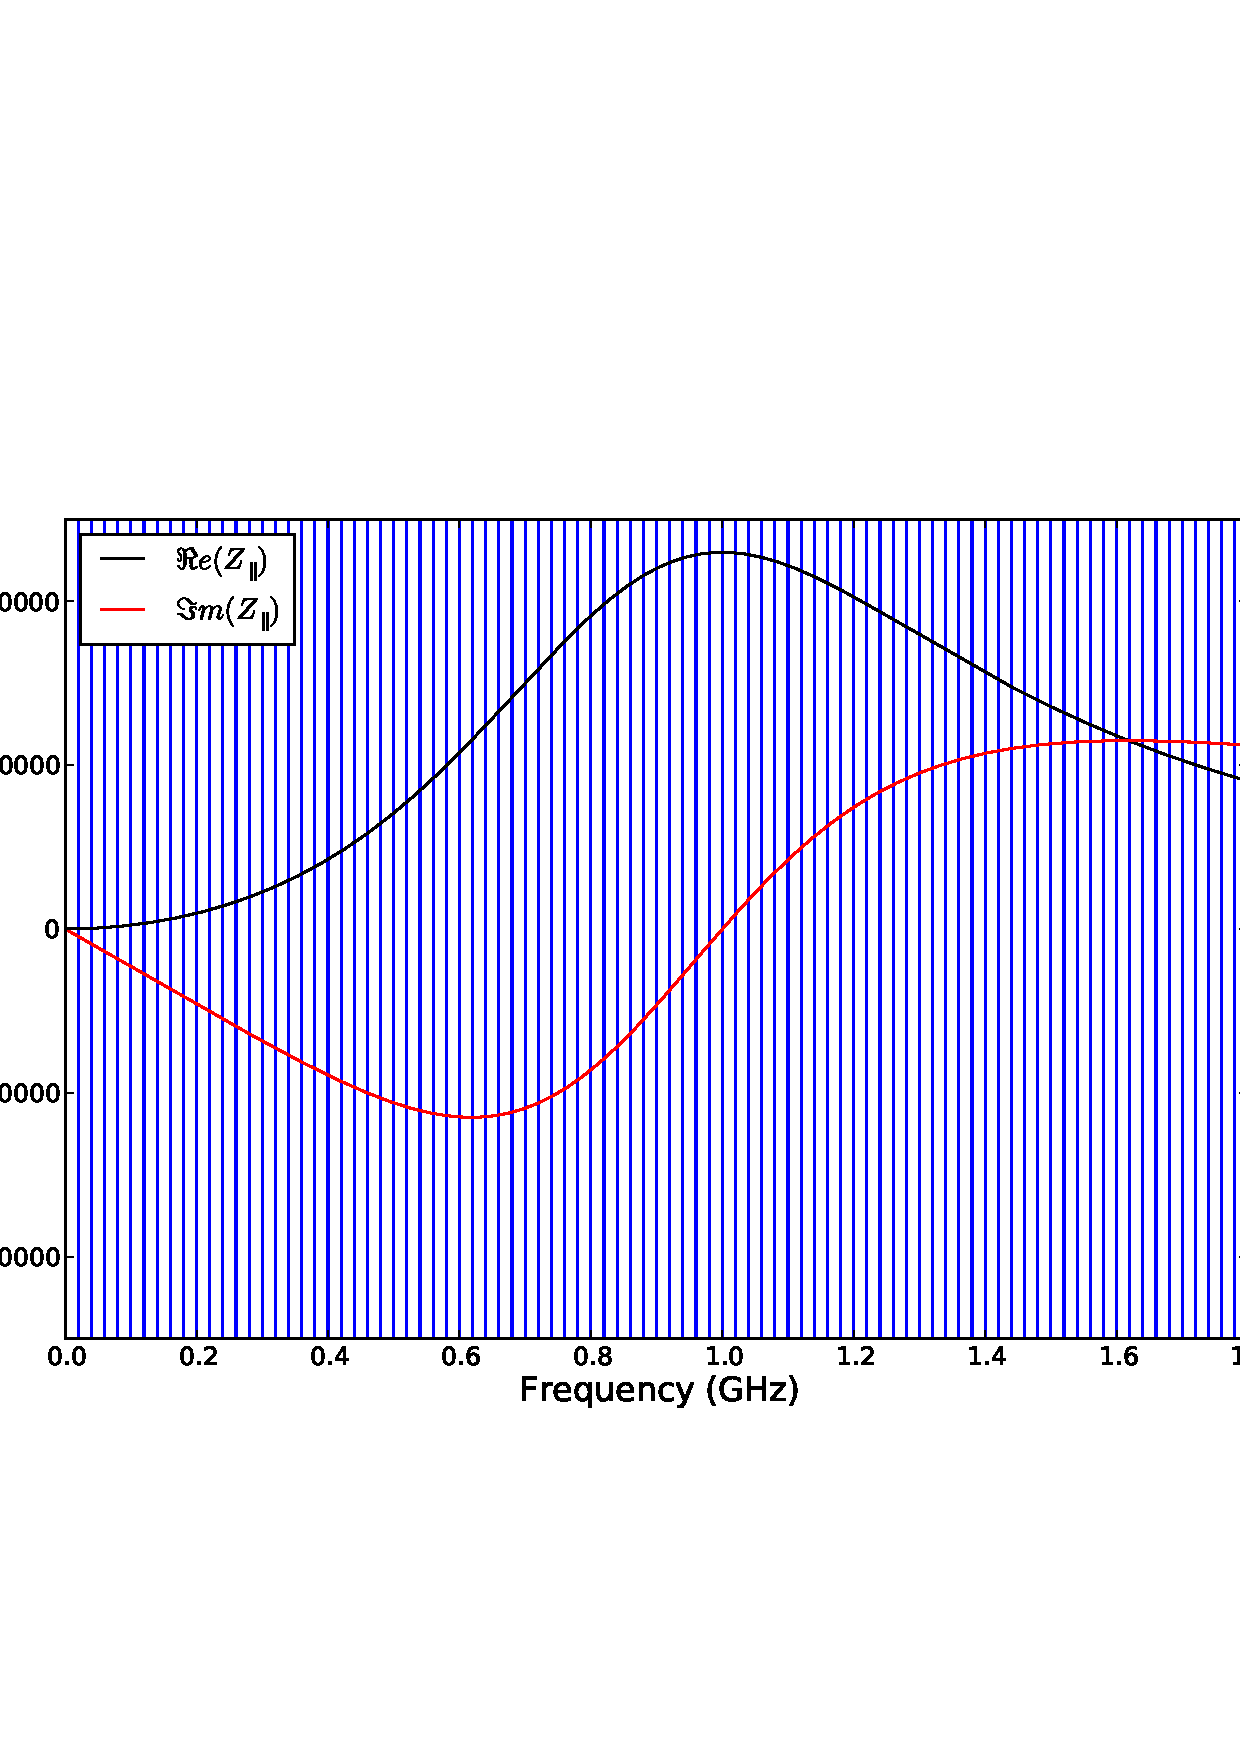
\includegraphics[width=0.75\textwidth]{figures/wakefields_and_impedance/50ns_bunch_spacing_spectral_lines.pdf}
\label{fig:BB-20MHz-spacing}
}
\subfigure[]{
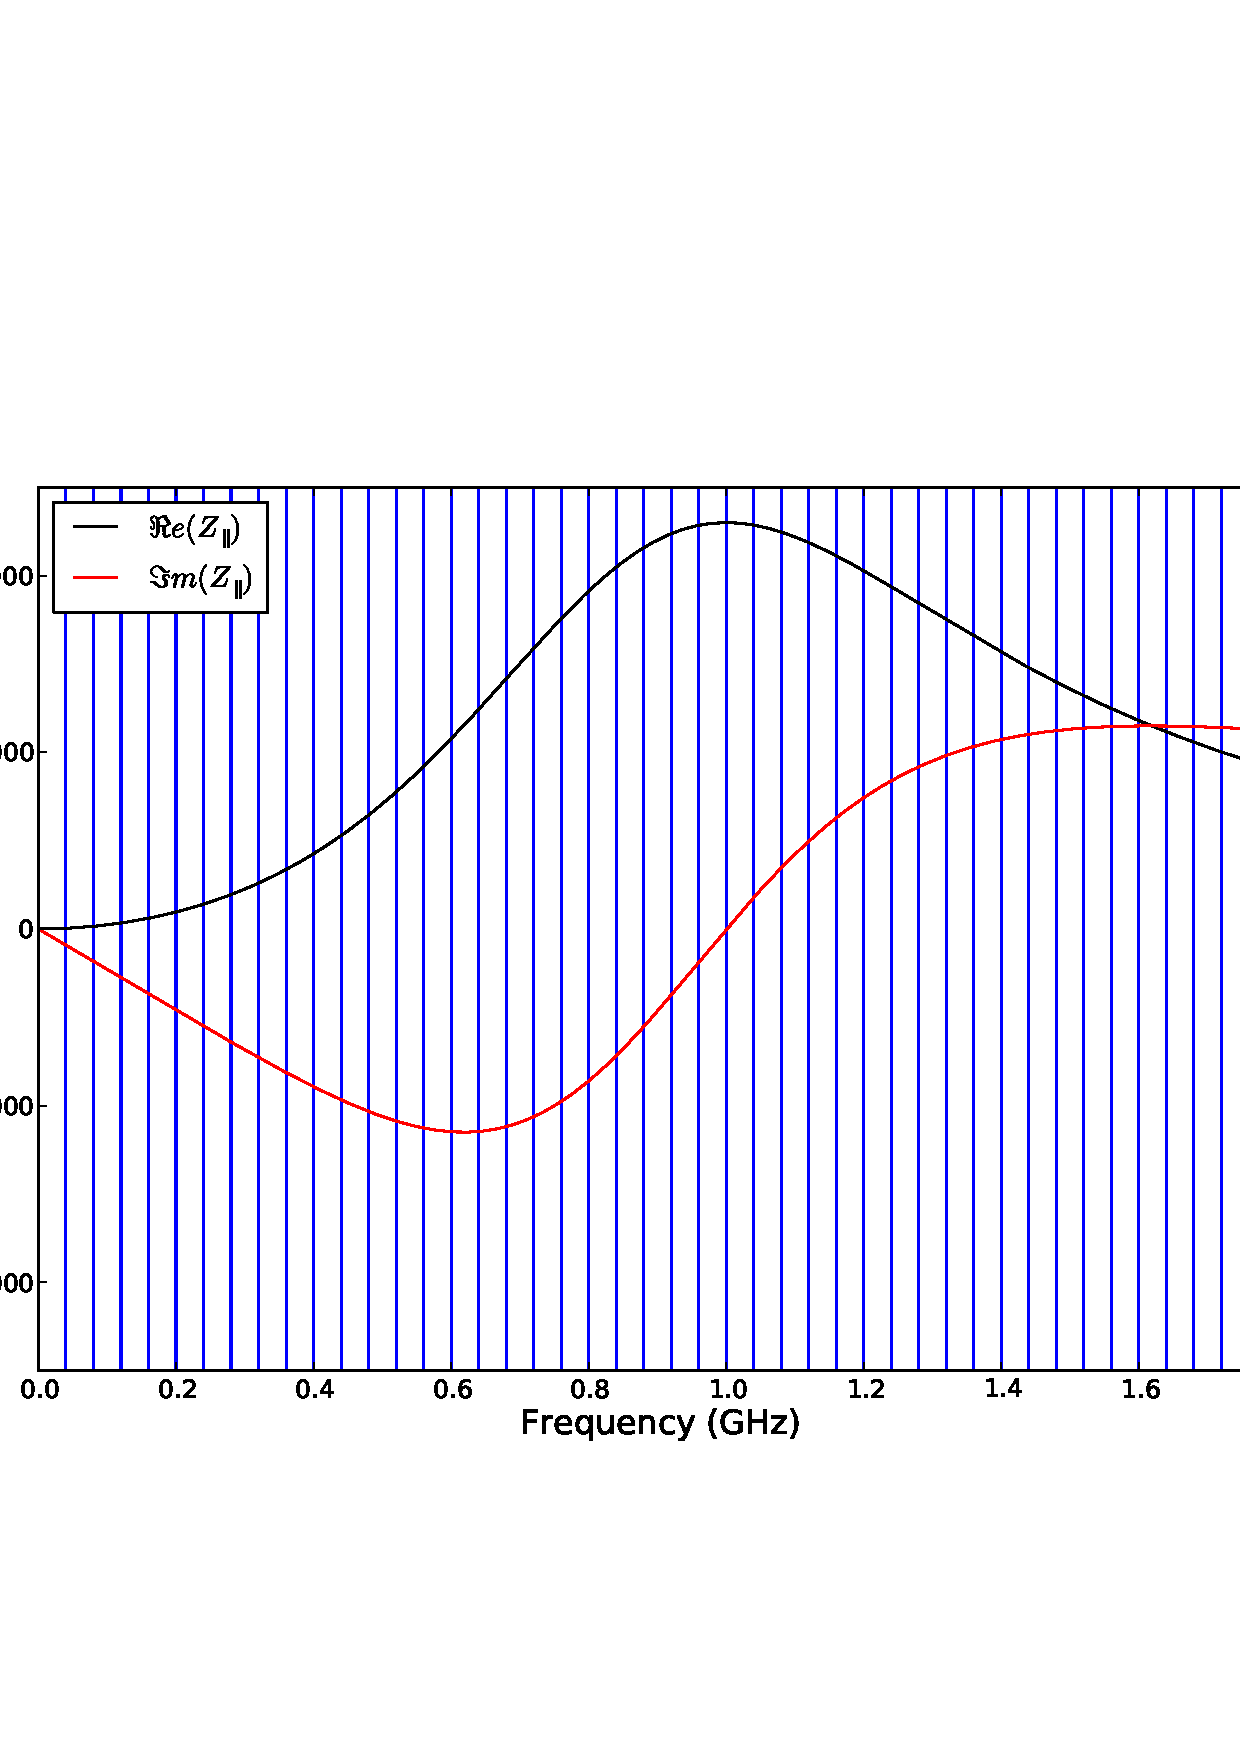
\includegraphics[width=0.75\textwidth]{figures/wakefields_and_impedance/25ns_bunch_spacing_spectral_lines.pdf}
\label{fig:BB-40MHz-spacing}
}

\end{center}
\caption{The spectral lines of a beam with \ref{fig:BB-20MHz-spacing} 50ns bunch spacing and \ref{fig:BB-40MHz-spacing} 25ns bunch spacing with a broadband impedance ($R_{s} = 0.23M\Omega, Q=1, \omega_{0} = 1$GHz)}
\label{fig:spectral-lines-BB}
\end{figure}
\begin{figure}

\caption{The change in power loss due to a broadband impedance with an increased  number of bunches in a storage ring}
\end{figure}


%% Example done with a low Q (Q ~ 1/10)
%% To illustrate effect of bunch length increase
Note that technically the increase is linear with number of bunches due to the increase seperation of spectral lines

\subsubsection{Heating due to a Narrowband Impedance}

For narrow band impedances (Q$\gg$100) which lie upon a single spectral line (i.e. $\omega_{res} = mn_{bunch}\omega_{0}$, where m is some integer) we can see that the power loss due to this spectral line becomes from Eqn. \ref{eqn:heating-gen}

\begin{equation}
P_{loss}  = \left( \omega_{rev}eN_{b}n_{bunch}  \right)^{2} \left( 2 \left| \lambda \left( \omega_{res} \right)  \right|^{2}  \Re{}e \left( Z_{\parallel} \left( \omega_{res}\right) \right) \right) 
\label{eqn:loss_narrow_band}
\end{equation}
%% Example done with a high Q (Q ~ 1000/10000) 
%% To illustrate bunch length changes (location of secondary hump)

\begin{figure}
\begin{center}
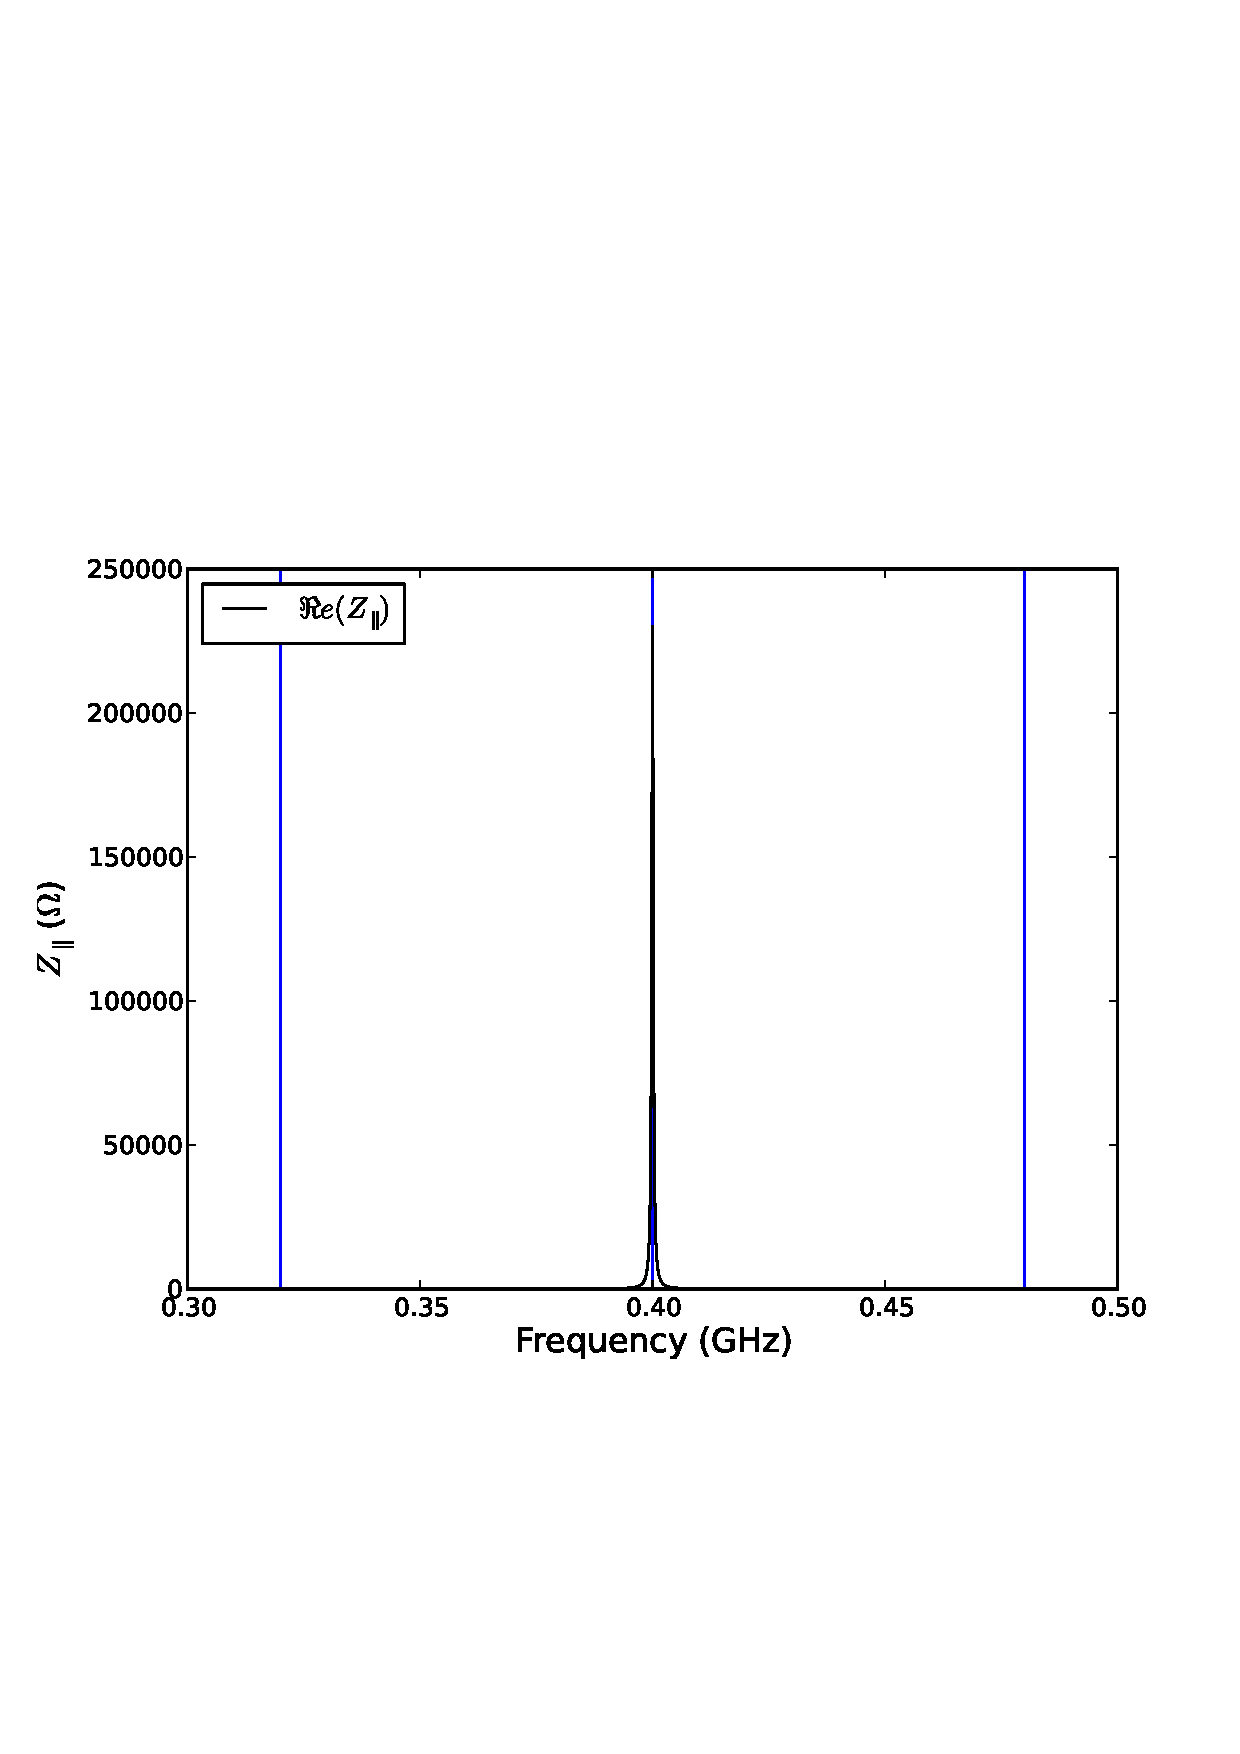
\includegraphics[width=0.7\textwidth]{figures/wakefields_and_impedance/impedance_narrow_band.pdf}
\caption{The spectral lines overlaying on a narrow band ilpedance. The spectral lines (in blue) are for $\omega_{0}=40\text{MHz}$. Note how only a single spectral line lies on this impedance.}
\label{fig:heating-high-q}
\end{center}
\end{figure}

\subsection{Single Bunch and Coupled Bunch Instabilities}

\subsection{Example of LMCI with Broadband and Space Charge Impedances Studied with HEADTAIL}

%
% Theory of LMCI (potential well distortion and microwave instability)
% Simulations with BB, SC and BB/SC impedances
% Comparison of different impedances and their production of different stability criteria
%